\section{Virtual microworlds}

Unlike our jamming and creative writing microworlds, Minecraft is a
\emph{virtual} microworld. This means that software is an integral part
of the microworld, in a way that is not necessarily true for mostly
physical microworlds.

How does software change things? It eliminates routine tasks, by
delegating those to the machine. Let's see how that works in practice:

The physical microworld equivalent of Minecraft is a pile of Lego bricks
on the floor. Unlike Minecraft, everything is, understandably, manual.
The only way to search for certain kinds of bricks is by conducting a
linear search, or, if you're very organised, sorting the bricks first.

There is a limit to the number of bricks the average person can handle.
This limits the complexity of our Lego creations. There are also
constraints of time and space.

Playing with Lego can occupy the entire floor. This means that only
those people with access to the floor can play. Even at the most social
Lego sessions, it's unlikely more than a handful of people will be able
to participate simultaneously.

And before long, the Lego will have to be tidied away. As bricks are
physical, this usually entails breaking up any structures and putting
single bricks back in the box.

Minecraft is different. As the bricks are virtual, they can be sorted
and organised by the machine. They can be practically infinite in
number, and the increasing complexity in structures can be handled by
the user interface treating a grouping of blocks as one.

The environment is virtual too, so bricks don't have to be tidied away
when you're done; their patterns are stored in bits until you're ready
to return. This makes it easier to work on larger-scale projects, as it
eliminates the need to ever start over from scratch.

It also makes it easier for users to collaborate. Builders no longer
have to be friends, or even geographically close to each other, to work
together in the same environment. They just need to be logged in to the
same server. This encourages large-scale collaborative projects.

But software also creates a barrier to entry. To participate in a
virtual microworld, you need specialised equipment - a computer - that
can run it. That said, you need specialised equipment, such as musical
instruments, to participate in physical microworlds too, and it seems
that computers are becoming less and less ``specialised'' as time goes
on.

However, to run a virtual microworld, you also need specialised
\emph{software} to go along with your hardware. For Minecraft, you need
to install the Minecraft software package. For programming microworlds,
you often need to install an interpreter, configure an editor and to set
up a build system.

The easier a microworld is to enter, the greater its potential audience.
The microworlds that are easiest to enter require the least set up of
specialised software on the part of the user.

The web browser is fast becoming less and less specialised. All
computers come with them pre-installed, and most users spend a
significant part of their computer time using them.

Microworlds in the web browser are arguably the most easily accessible
virtual microworlds. Let's take a look at some current examples.

\subsection{CodePen (\href{http://codepen.io/}{http://codepen.io/})}

CodePen is a browser-based virtual microworld for front-end web
development, i.e.~HTML, CSS and JavaScript. The creation view looks like
this:

\begin{figure}[ht!]
\centering
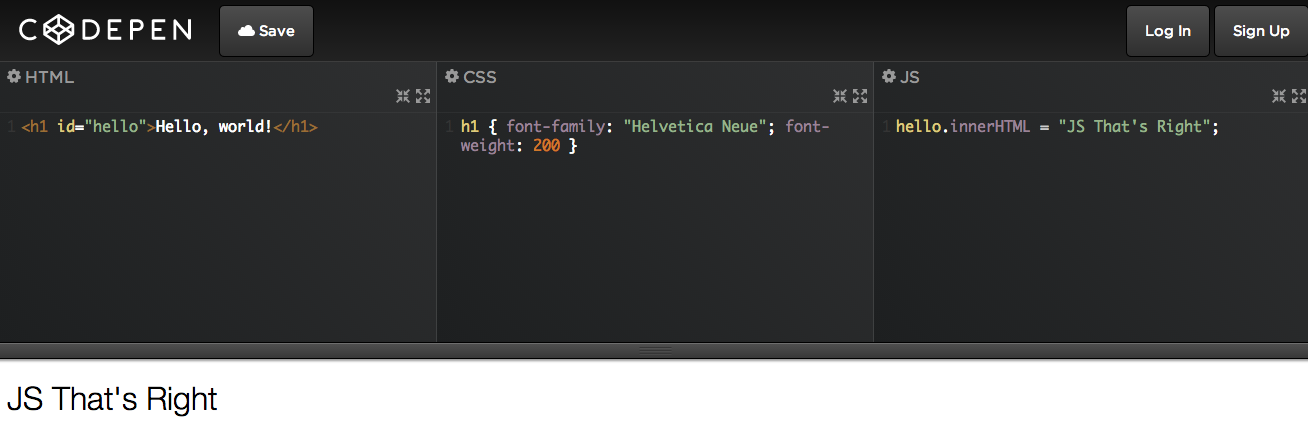
\includegraphics[width=123mm]{img/codepen.png}
\caption{CodePen interface}
\label{overflow}
\end{figure}

There are four panes: one each for HTML, CSS and JavaScript code, and
one that dynamically renders the result.

This microworld leverages the browsers capacity for dynamic rendering:
of parsing and showing the results of code on the fly. A website allows
you to experiment with creating websites.

Created entities in CodePen - ``Pens'' - are public entities and can be
browsed by others, and even tweaked by them. This creates a rich
environment for creativity and experimentation, and as we have argued so
far, a rich source of learning, in this case in the domain of front-end
web technology.

\subsection{Pacemaker (\url{http://pacemaker.net/})}

Pacemaker is an iPad application that is also a virtual, musical microworld. It enables users to remix and edit songs from Spotify, in real-time, by touching the iPad screen.

\begin{figure}[ht!]
\centering
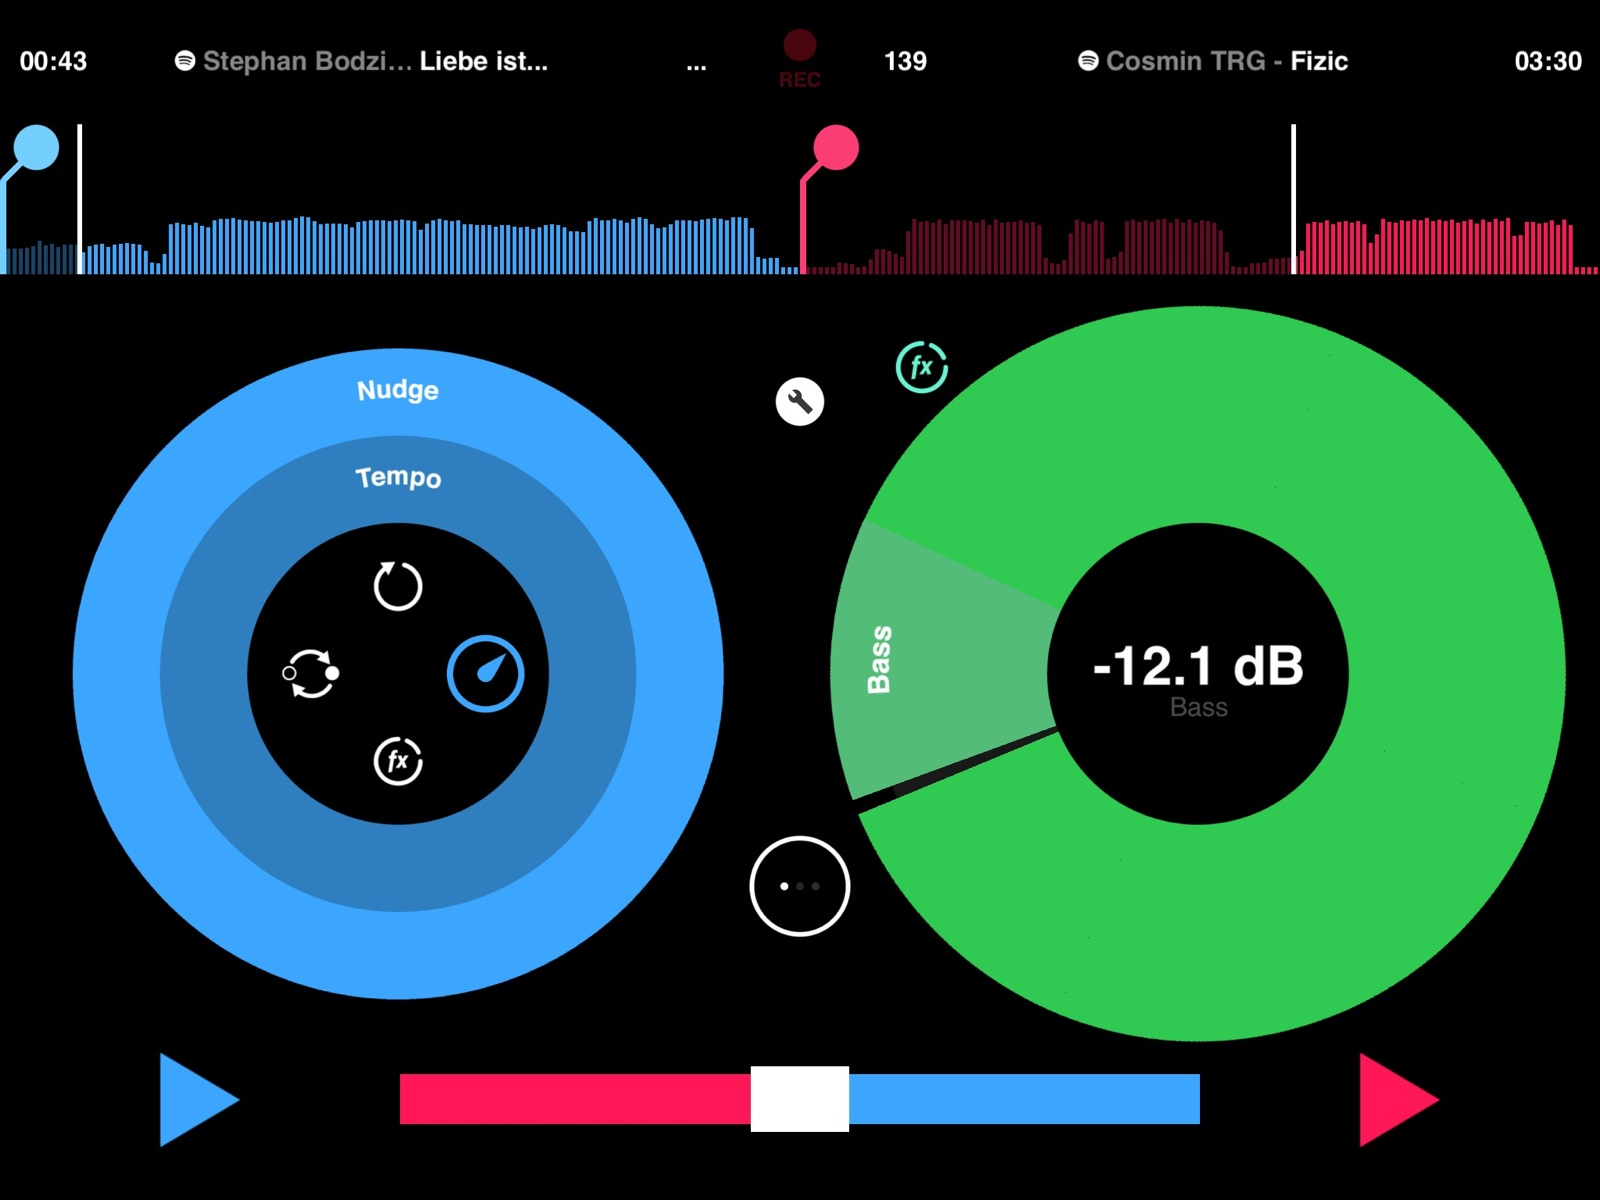
\includegraphics[width=123mm]{img/pacemaker.jpg}
\caption{Pacemaker interface}
\label{overflow}
\end{figure}

Sadly, Pacemaker does not allow sharing of creations, due to copyright issues. But creations can be played back on the iPad that created them so that listeners can evaluate them. 

\subsection{Blogging}

There are many blogging systems on the internet, such as \href{http://wordpress.org/}{Wordpress}, \href{http://tumblr.com}{Tumblr}, \href{http://medium.com}{Medium} and \href{http://ghost.org}{Ghost}. 

Blogging is a virtual microworld where \textbf{ideas} are \textbf{implemented} as text and images, and then (hopefully) \textbf{evaluated} by readers who give feedback by sharing and commenting about blog posts on social media. 

\begin{figure}[ht!]
\centering
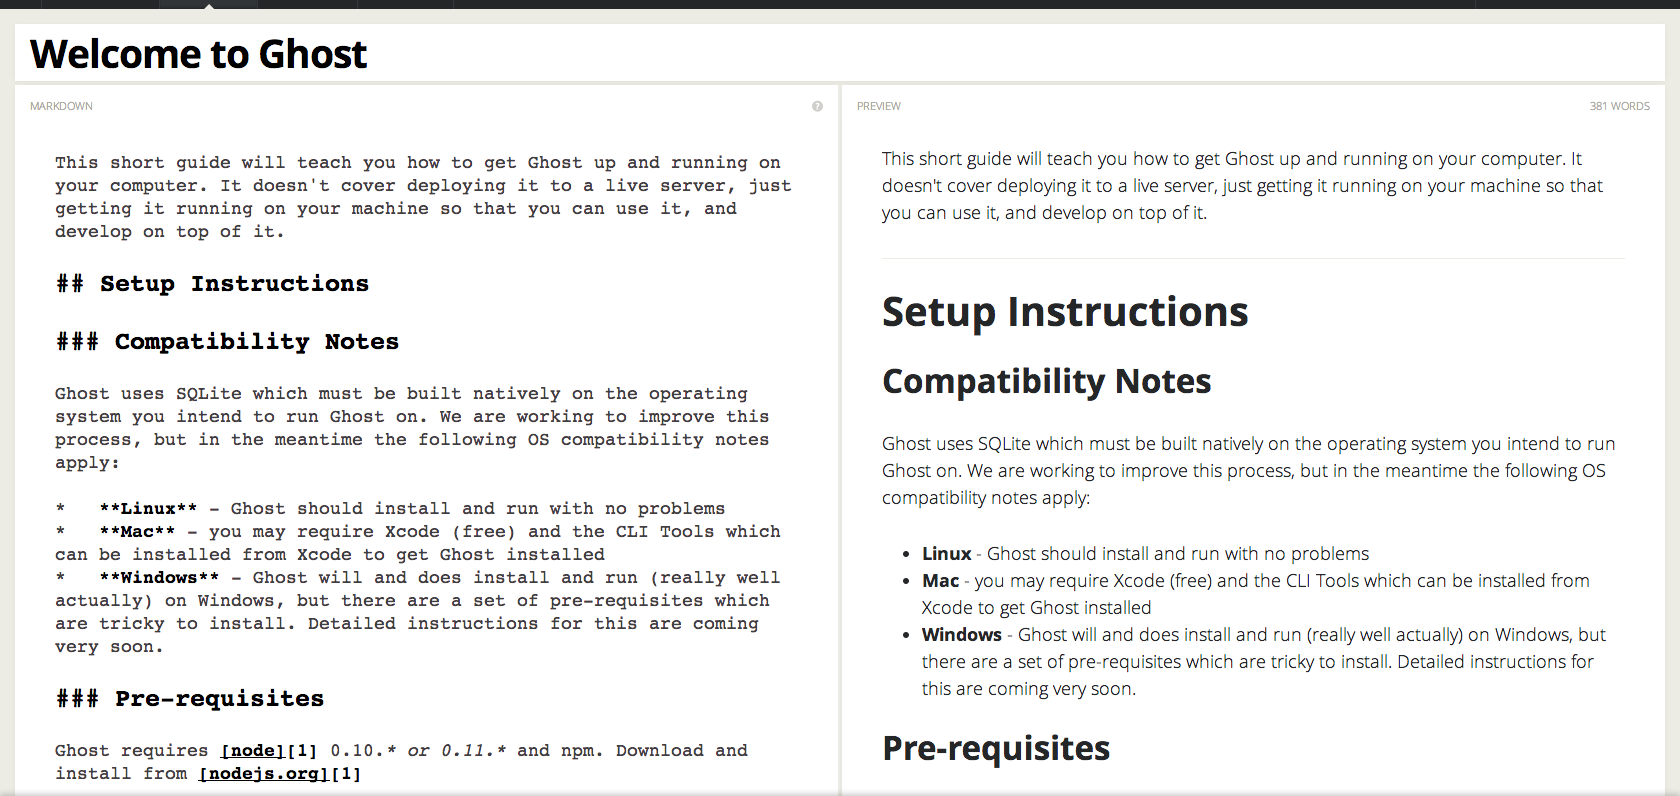
\includegraphics[width=123mm]{img/ghost.png}
\caption{Ghost editing interface}
\label{overflow}
\end{figure}

\subsection{A microworld for microworlds}

According to contructionism, and our sources from the last chapter, the best way for a person to learn about a domain is to construct public entities in that domain. Therefore, the best way for me to learn about microworlds is to build some myself. For the reasons outlined above, I chose to build virtual, browser-based microworlds. 

The next chapter describes these microworlds. 
